\documentclass[main.tex]{subfiles}
\begin{document}
	然后单击 Spyder 下面的 Launch 就会打开 Spyder。单击 Jupyter 下面的 Launch 就会打开 Spyder
打开 Spyder
\begin{figure}[h]
	\centering
	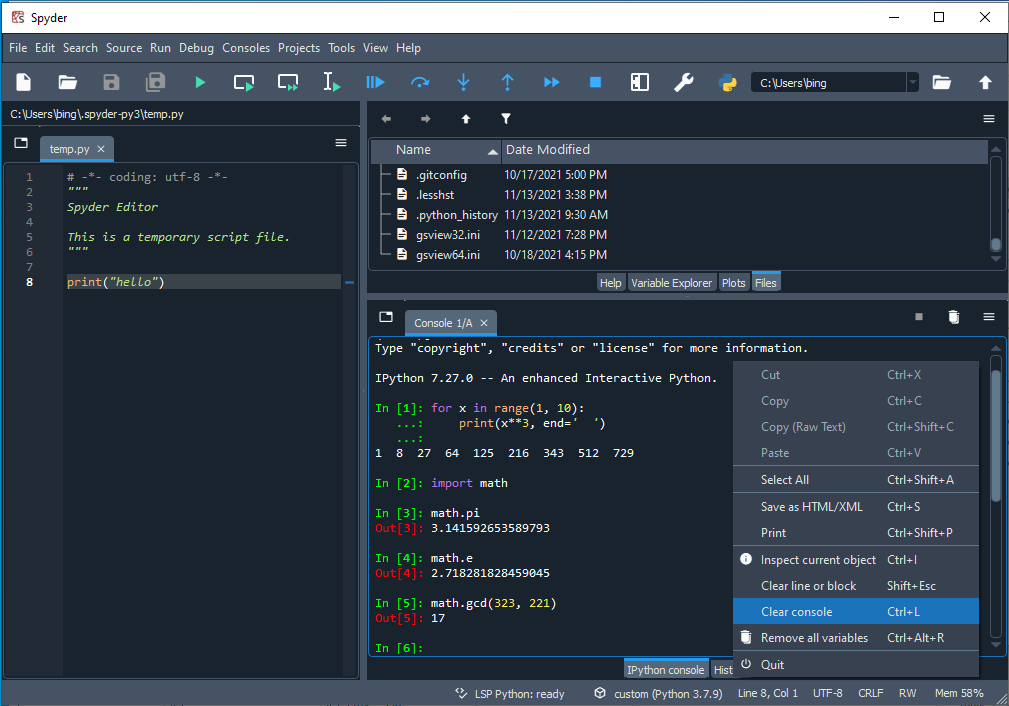
\includegraphics[width=1.0\textwidth]{png/spyder_ide.png}
	\caption{Spyder IDE}
	\label{fig:2.3.1}
\end{figure}


the Specifying Colors tutorial;
the matplotlib.colors API;
the Color Demo.
\begin{verbatim}
	Text enclosed 'inside' \texttt{verbatim} environment 
	is printed directly 
	and all \LaTeX{} commands are ignored.下面的 
\end{verbatim}

\begin{spacing}{0.8}
\begin{small}
\begin{lstlisting}[language=Python]
import re

x = "100以内有25个质数。"
x += "不实际计算的话,51和91很容易被误判为是素数。"
y = re.sub("质数", "素数", x)
z = x.replace("素数", "质数")
print(y)
print(z)
print(x)

#%%
import math

print("hello")
print(re.sub("This", "That", "This is not"))
print(math.pi)
\end{lstlisting}
\end{small}
\end{spacing}


\end{document} 
